\section{Methodology}

\subsection{Model}

We assume an application model that is similar to Secret~\cite{secret}.
\begin{figure}
\centering
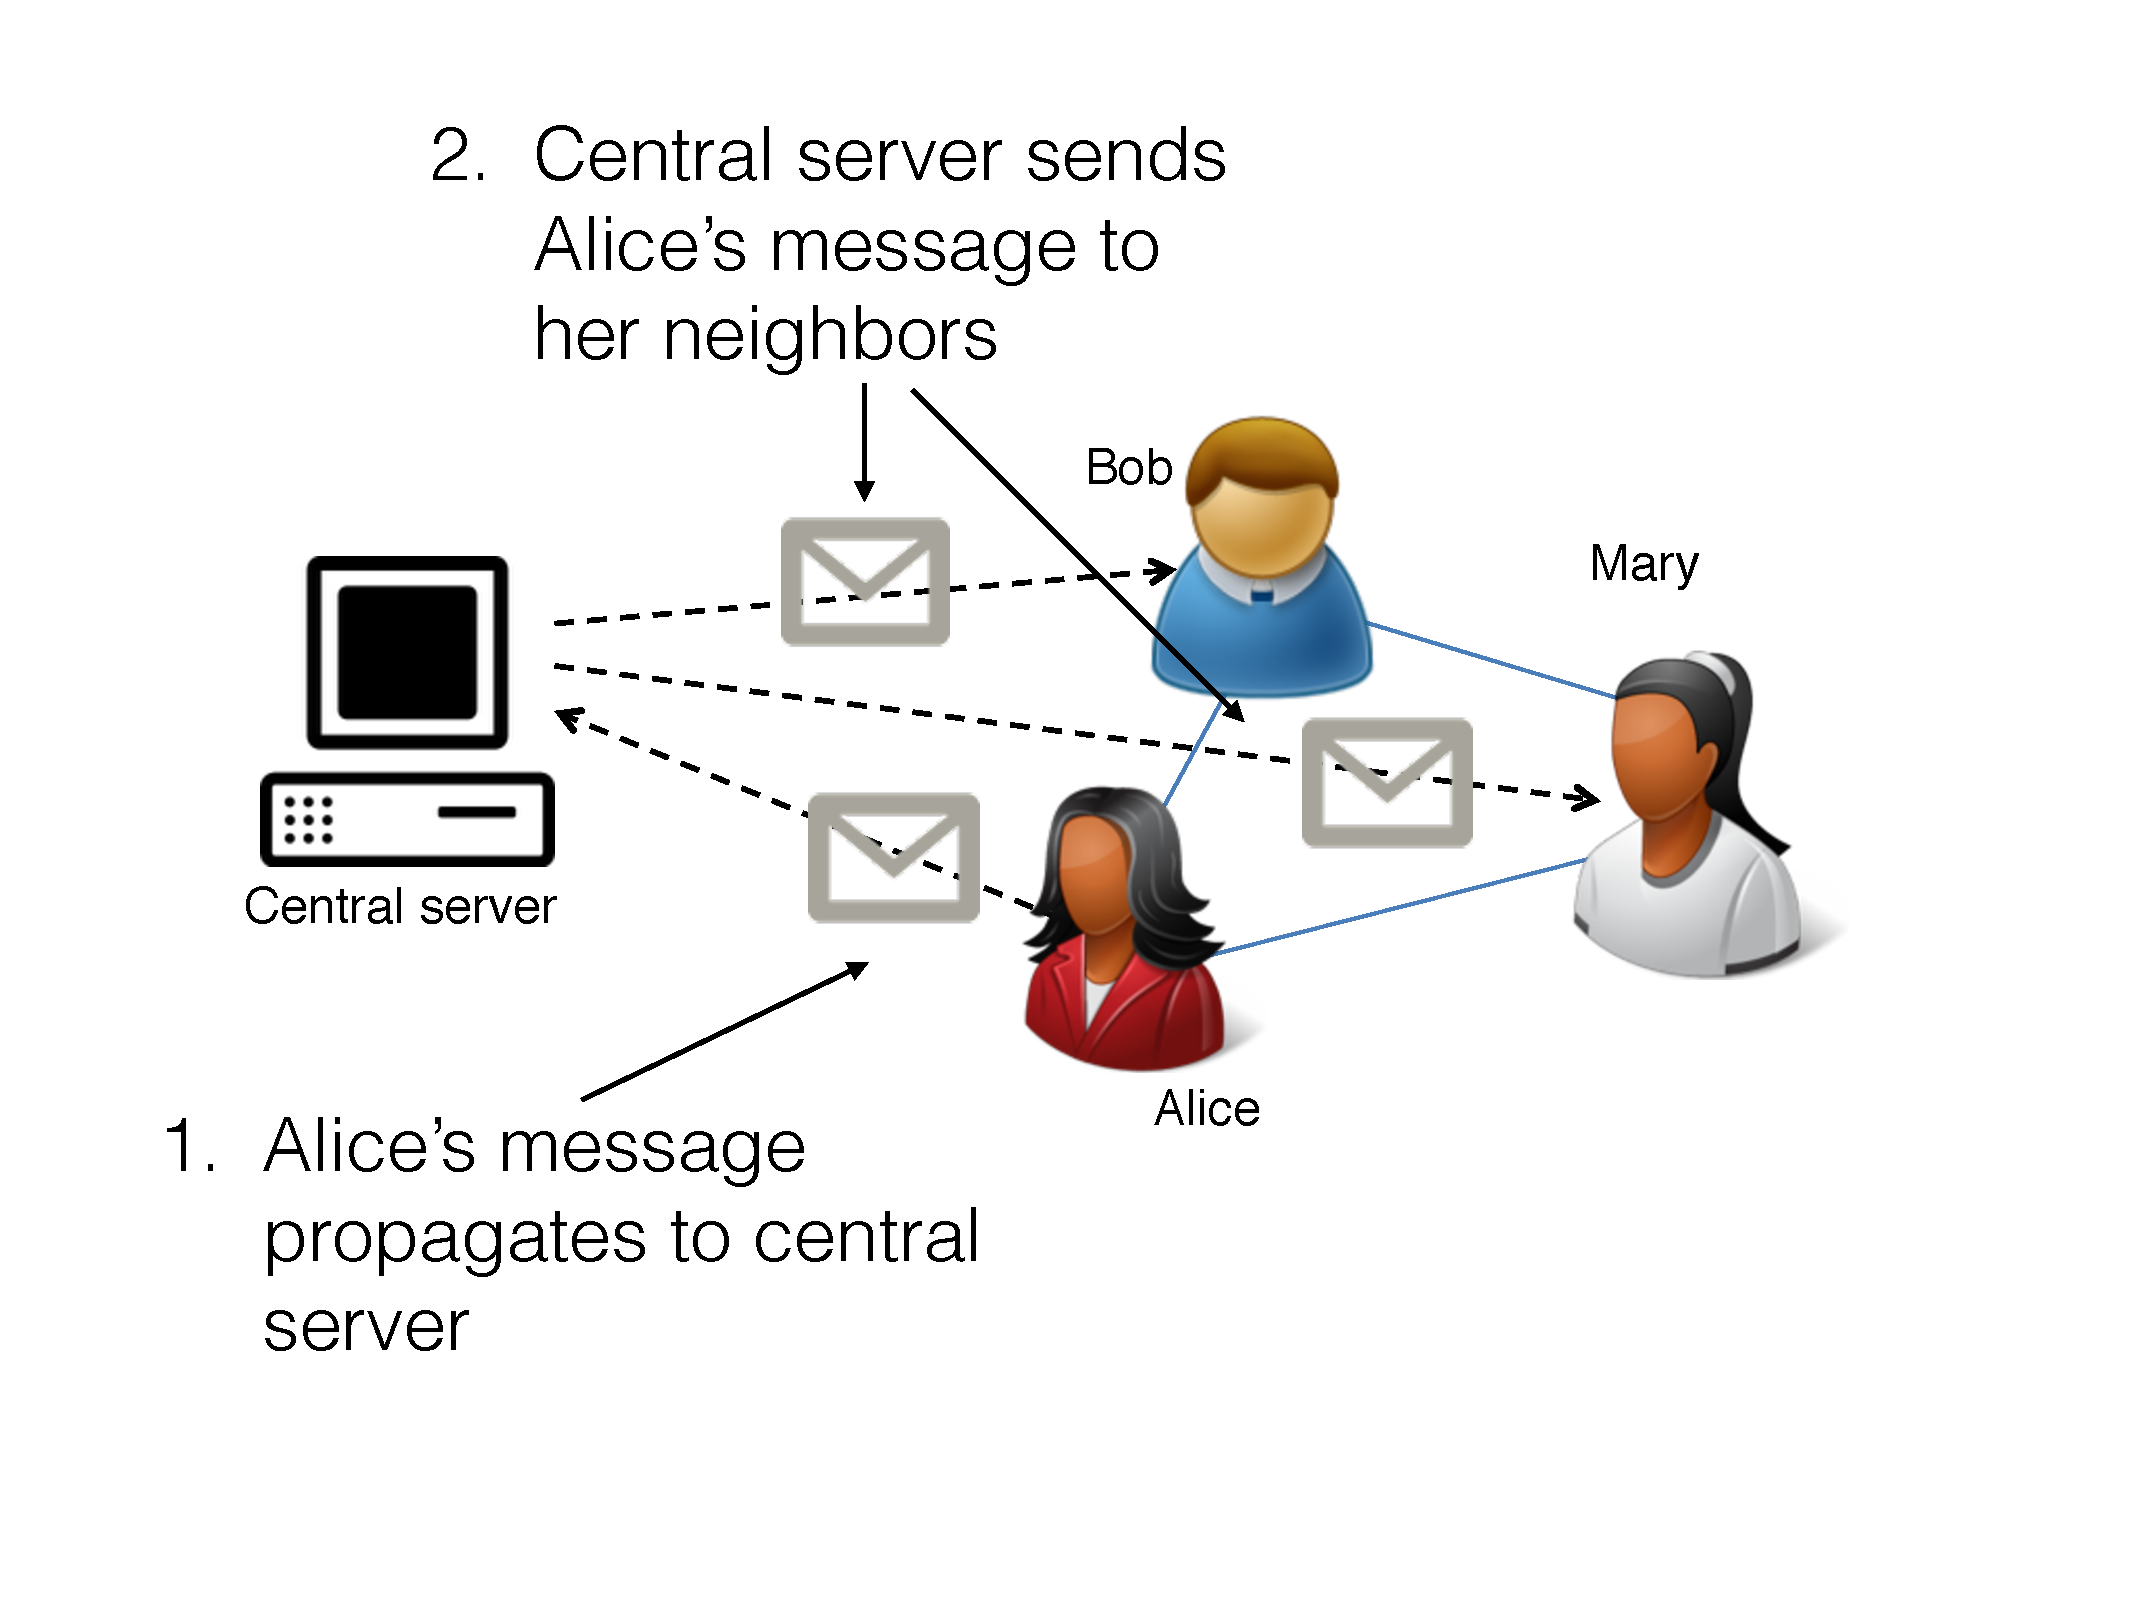
\includegraphics[height = 2.4in]{figures/secret_infrastructure}
\caption{An overview of the infrastructure for a typical anonymous social network.}
\label{fig:secret_infrastructure}
\end{figure}
Fig.~\ref{fig:secret_infrastructure} shows how a typical anonymous microblogging network works. Users are connected to friends as in a regular social network; we model this social network as a graph $\mathcal G(V,E)$, where $V$ denotes the set of vertices, or participants, in the network, and $E$ denotes the set of edges. When a source node, Alice, decides to send a message to her friends, her message is routed to a centralized server first. We denote the source node by $v^*$. The server propagates the message to Alice's neighbors, $\mathcal N(v^*)$. Alice's neighbors do not know who sent or authored the message. %To them, the message is from the centralized server instead of directly from Alice, and does not have any information about the sender herself. 
If one of Alice's friends decides to ``like'' the message, the message will be further propagated to her friend's friends. Thus, whenever a user receives a message, he/she does not know if a neighboring friend sent it, or if it was simply liked by a friend. We assume that propagation occurs with some time delay, which captures the time between the server pushing a message and the receipient actually seeing it. We model the delay between a user $i$ liking a message and the user's friend $j$ seeing the message as a random variable $\theta_{ij}$; the $\theta_{ij}$'s, or delays across each edge in the social graph, are assumed to be iid random variables. We do not specify the distribution of $\theta_{ij}$ \emph{a priori}; in principle, this should be informed by measurements of real social network usage.

Our adversarial model considers a moderately powerful adversary that is able to compromise certain users in the social network. This might occur by offering incentives to users and recruiting them to act as spies. The spies are not active, but are instead passive observers. The only thing that differentiates spies from honest users is that spies collect all observed messages (along with timestamps), and then send this information to the adversary. The adversary uses the collected message timetamps to attempt to track down the perpetrator of the message.
We assume there are $K$ spies in the network, $o_1,\ldots,o_K$. For a given message $m$, each spy $o_i$ will collect the timestamp $t_i^{(m)}$ at which it first receives the message. The adversary must then output an estimate $\hat v$, which it believes to be the true source of message $m$. %Therefore, the 

The central adversary will receive different sets of messages, and it will need to group them into a \emph{collection} -- a group of messages received at different nodes that came from the same source. We assume that these messages are not encrypted, and thus the adversary can use the plaintext information directly to identify the correct collection membership. 

\subsection{Efficacy of deanonymization}

We study the ability of this adversary to deanonymize users through simulation. A number of factors could impact deanonymization:

\begin{description}
\vspace{-0.1in}
\item[Underlying graph structure:] The underlying graph structure can significantly affect deanonymization. For example, a tree-like structure with no loops is easier to deanonymize because there are fewer possible paths between nodes to analyze. In our simulation, we study a range of graph structures, including trees, Erdos-Renyi, and Barabasi-Albert graphs.
\item[Fraction of spies:] The fraction of spies will greatly impact the deanonymization performance. Fewer spies means less information, and thus makes the true source much harder to track. Using simulation, we want to \emph{quantify} how many spies are needed to efficiently find the true source.
\item[Location of spies:] We hypothesize that selecting spies as high-degree nodes will increase the probability of detection, as popular nodes are more likely to see and propagate the message. However, this may be unrealistic in practice, as popular individuals (i.e., high-degree nodes) may hold more social leverage and may therefore resist recruitment attempts. A uniform distribution of spy nodes seems feasible for an adversary with moderate but limited resources. 
\item[Propagation latency:] The propagation latencies $\theta_{ij}$ are likely to depend on many factors, such as the popularity of the social network, the habits of its users, and the application platform (e.g., mobile vs. desktop).
In simulation, we model the propagation latency in two ways: using a Gaussian distribution with a high mean-to-standard-deviation ratio, and a geometric random variable. 
\item[Estimator:] To maximize probability of detection, i.e. $P(\hat v=v^*)$, the adversary should use a maximum-likelihood (ML) estimator. However, computationally-efficient ML estimators are not known for general graph structures and propagation delay models. We therefore try different methods of estimation. The majority of our effort goes towards adapting the estimator in~\cite{pinto} to our spy-based adversarial model.
\end{description}

\subsection{Estimators}
Initially, we attempted to come up with some estimators on our own. \todo{Should we mention the Jordan estimators here?}



\subsubsection{ML estimator for trees}
The observer model estimator~\cite{pinto} is a maximum likelihood estimator. The setup is quite similar to our simulation: given a graph $\mathcal G$, there exists a set of $K$ observers that observe information transmitted in the network. The collected information has a timestamp, as well as direction information (e.g. observer $o$ receives the message from neighbor $v$). This is the main difference between \cite{pinto} and our work; we do not assume that spies have direction information. \cite{pinto} also assumes that propagation delays are modeled by iid Gaussian random variables with distribution $\mathcal N(\mu,\sigma^2)$. We start by defining some terms:

Let $\boldsymbol{d}$ be the timestamp differences of observed arrivals with respect to some reference spy node, defined as
\begin{equation}
  \boldsymbol{d}_k = t_{k} - t_1
\end{equation}
where $t_i$ denotes the observed timestamp at spy $i$, and $k = 2,\ldots, K$.

The next term is the expected delay, which is the delay that one \emph{should} observe if the information had propagated from some candidate source $s$ ($s$ is an honest node in the graph):
\begin{equation}
  \boldsymbol{\mu}_{s,k} = \mu (|P(s, o_{k+1})| - |P(s, o_1)|)
\end{equation}
where $|P(u, v)|$ denotes the number of edges on the path that connects nodes $u$ and $v$. Finally, we define a scaled covariance matrix, which represents the covariance of the jointly-gaussian delay random variable:
\begin{equation}
  (\boldsymbol{\Lambda}_s)_{k, i} = \begin{cases}
    |P(o_1, o_{k+1})| & \text{if $k = i$} \\
    |P(o_1, o_{k+1}) \cap P(o_1, o_{i+1})| & \text{if $k \neq i$}.
  \end{cases}
\end{equation}
$\boldsymbol \Lambda_s$ does not depend on $s$ when $\mathcal G$ is a tree. However, for general graphs, there may be multiple paths between a pair of nodes. As such, \cite{pinto} suggests that all paths should be computed over a breadth-first-search tree rooted at the candidate node $s$.

The authors use these terms to construct a source estimator for general trees:
\begin{equation}
\label{eq:general}
\hat{s} = \arg\max_{s \in \mathcal T_{a}} \dfrac{\exp(-\frac{1}{2} (\boldsymbol{d} - \boldsymbol{\mu}_{s})^{T} \boldsymbol{\Lambda}_s^{-1} (\boldsymbol{d} - \boldsymbol{\mu}_s) }{|\boldsymbol{\Lambda}_s|^{1/2}}.
\end{equation}

$\mathcal T_a$ denotes the \emph{pruned} tree. Pruning refers to the process of removing nodes from $\mathcal G$ that could not have possibly generated the observed information. For instance, consider Figure \ref{fig:pruning}; the spies $o_1$ and $o_2$ both observe that they received the message from node 3. Therefore, node 1 could not possibly have been the source, and we can prune it from the tree. In this example, the pruned tree $\mathcal T_a$ consists solely of node 3. For trees, this pruning process does not change the probability of detection; it only speeds up estimation. However, we will show later that for loopy graphs, pruning significantly increases the probability of detection. In scenarios where direction information is not available (as in our application), we cannot prune, and therefore have lower detection accuracy.

\begin{figure}[h]
\centering
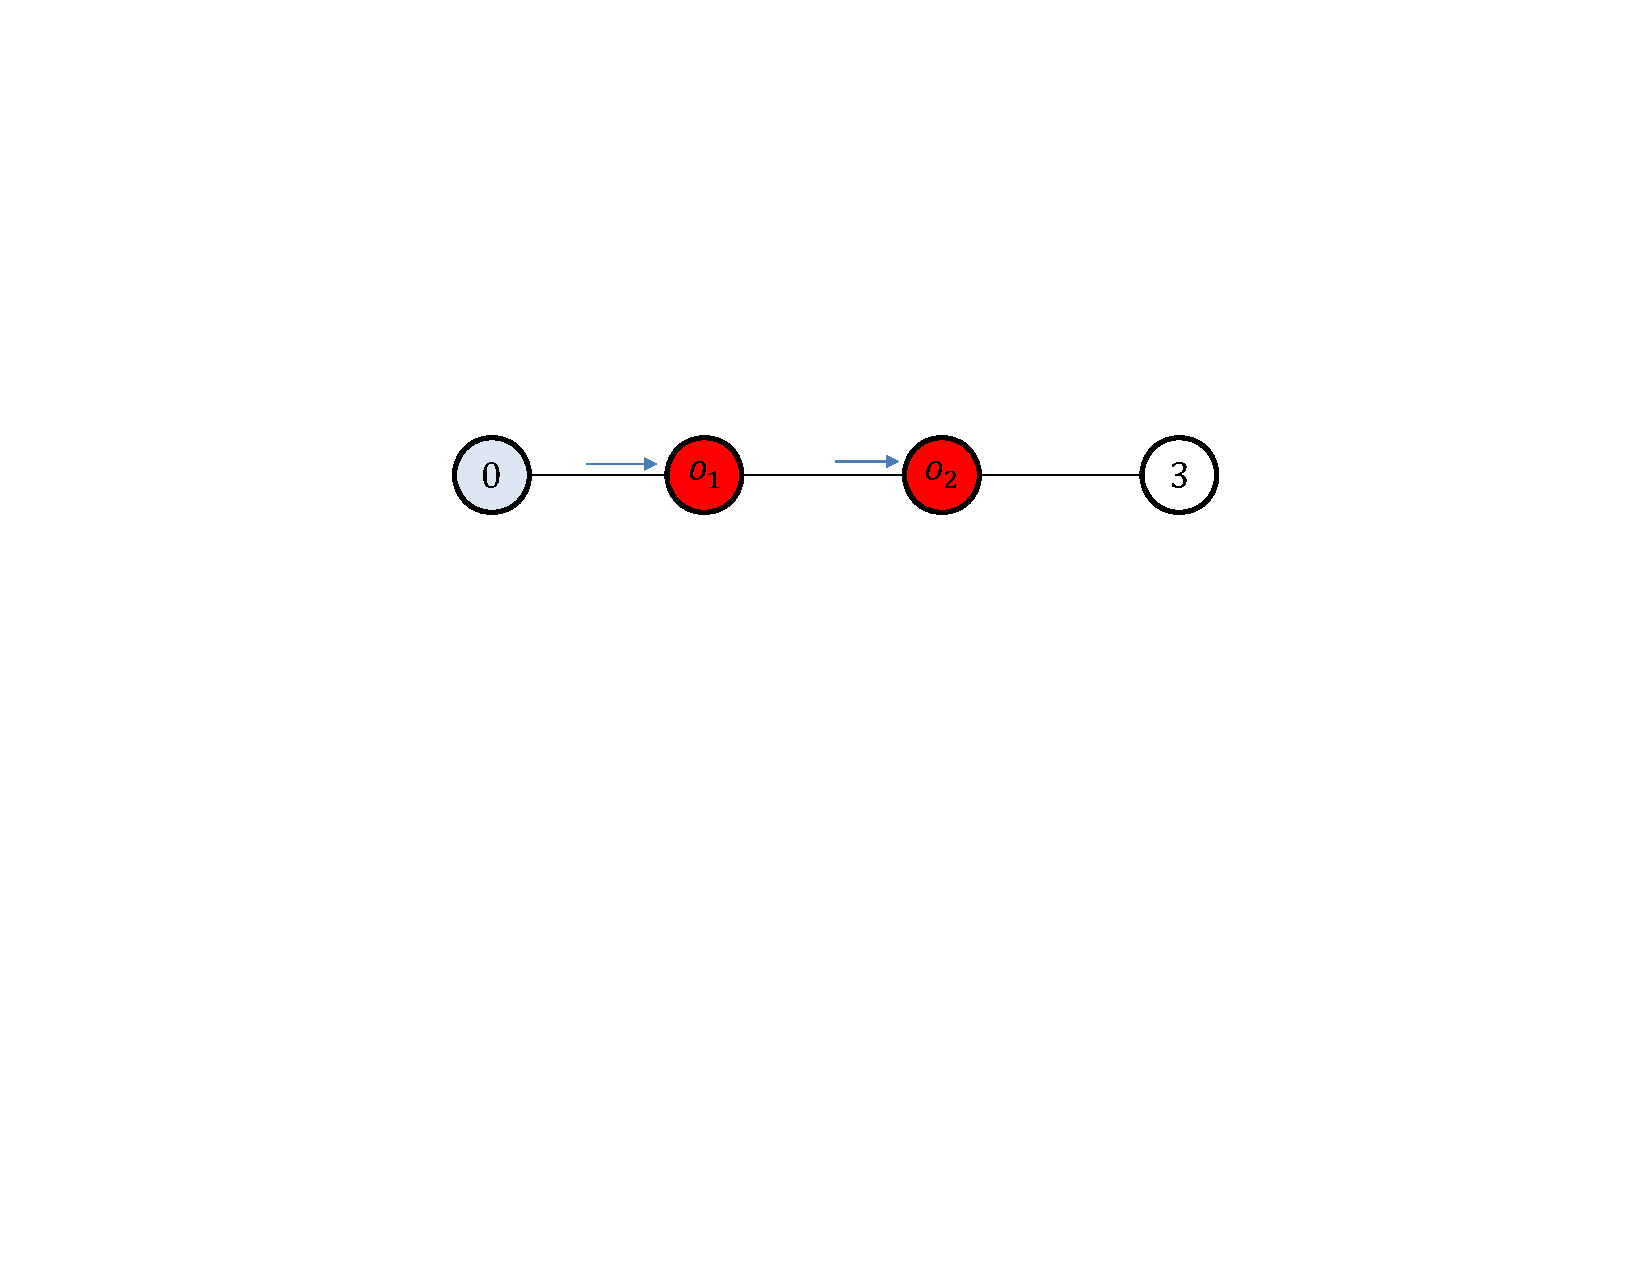
\includegraphics[width = 3.2in]{figures/pruning}
\caption{Directionality information enables the adversary to remove nodes that could not have generated the spies' observations. In this example, the pruned tree $\mathcal T_a$ consists only of node 3.}
\label{fig:pruning}
%\vspace*{-0.4in}
\end{figure}


Equation \ref{eq:general} can be applied to general graphs as a heuristic estimator. However, if the underlying graph is tree-structured, equation \ref{eq:general} simplifies to
\begin{equation}
\label{eq:tree}
\hat{s} = \arg\max_{s \in \tau_{a}} \boldsymbol{\mu}_{s}^{T} \boldsymbol{\Lambda}^{-1} (\boldsymbol{d} - \frac{1}{2}\boldsymbol{\mu}_s).
\end{equation}
because $\Lambda_s$ is constant for all candidate nodes. This estimator is provably optimal for tree-structured graphs.

\subsubsection{First-spy estimator}
We also tested a heuristic baseline estimator, which uses only partial spy information. This `first-spy' estimator considers only the first spy to receive the message, i.e., the spy with the smallest timestamp. Without loss of generality, assume that spy is $o_1$. The estimator chooses $\hat s$ uniformly among the honest neighbors of $o_1$. This estimate does not use direction information to prune candidates. A trivial extension \emph{with pruning} instead chooses the node that delivered the message to the first spy. We compare this first-spy estimator with pruning to the estimator in \cite{pinto}, which also uses direction information. 